
\subsection{Project planning}
The projects course started in August 2020 and continued until mid January 2020 with the project deadline in the middle of December. To have a good structre and of the things to be done and synchronizing all the parts a plan was made to have a good overview of the project, shown in Table \ref{tab:overall_time_plan}. This plan enabled the group to be eflexible while still have a good long-term structure of the project. Every month a more detailed time plan was made to facilitate the small changes, dlays etc. 
\begin{frame}
    \subsection{Time plan}
    \frametitle{Overall timetable}
    \begin{table}
        \begin{tabular}{| l | c | c | c | c }
            
            Sep & Oct & Nov & Dec \\
            \hline \hline
            Concept generation & Evaluation & Evaluation &  \\ 
            \hline
            Theory & Prototyping & Evaluation & Finishing up \\
            \hline
            Simulation & Evaluation & Evaluation & \\
            \hline
            Prototyping & Final Design & Evaluation &  \\
            \hline
 
        \end{tabular}
    \end{table}    
\end{frame}


\begin{frame}
    \frametitle{Time plan for September}
    \begin{table}
        \begin{tabular}{l | c | c | c | c }
        Subproject & Week 1 & Week 2 & Week 3 & Week 4 \\
        \hline \hline
            Arrowhead & Reading& Setup & API & Prototyping\\
            Movable base & Reading& Modeling & Simulation & Implementation\\
            Arm and grip  & Reading & Kinematics & Simulation& Prototyping\\
            Object detection & Reading & Testing & Prototyping & Evaluation\\
        \end{tabular}
    \end{table}
\end{frame}
For the group members to what task were to be done, the built in function of Issues on the souce control platform Github\textregistered \ enabled all the project group members to see what had to be done every week. A Milestone was created for each week and populated with issues. When an issue was finished it coul simply be closed. If the issue was delayed it showed clearly in the Issue overview which tasks had to be prioritized. 

\subsection{Source control}
To keep track of the different software implementation the projects souce control implements Git in one common repository \cite{repo}. The repository is where all source code and relevand 3D-files are located. This report is written in LaTeX with Git as source control. To make sure it's easy for all members to write their designated sections a workflow was designed to to minimiza merge conflicts while writing drafts as show in Fig. \ref{fig:git_workflow}. Without this flow the group members would experience merge conflicts after every push which would make it more complex and time consuming. 

    \begin{figure}
        \begin{center}
\resizebox{6.0cm}{!}{

\begin{tikzpicture}
    [align=center, auto]
    \node [computing] (start) {\textbf{CHAPTER\_descriptive\_filename.tex}};
    \node [computing, below= of start] (push) {Push to \textbf{/sections}};
    \node [computing, below= of push] (finished) {Finished?};
    \node [computing, below= of finished] (write) {Write on section}; 
    \node [computing, below= of write] (commit) {Commit};

    \node [computing, right= of finished, xshift=5em] (branch) {New branch \\ \textbf{REVIEW\_chapter}};
    \node [computing, below= of branch] (paste) {Paste section in \\ \textbf{/chapters/chapter.tex}};
    \node [computing, below= of paste] (pushb) {Push new branch};
    \node [computing, below=of pushb] (PR) {PR against \textbf{report-unsafe}};
    \node [computing, below= of PR] (review) {Wait for review};
    
    



    \coordinate [left= of push] (lrpush);
    \coordinate [left= of write] (lrwrite);
    \coordinate [left= of commit] (lrcommit);
    \coordinate [left= of finished] (lrfinished);
    \coordinate [right= of PR] (crPR);
    \coordinate [below= of crPR] (crreview);
    



    \draw [->] (commit) -- (lrcommit) -| (lrpush) -- (push);

    \draw [->] (start) -- (push);

    \draw [->] (push) -- (finished) -- node[midway, fill=white] {No} (write) -- (commit);

    \draw [->] (finished) -- node[midway, fill=white] {Yes} (branch);

    \draw [->] (branch) -- (paste) -- (pushb) -- (PR)  -- (review);

    \draw [->] (review) -| (crreview) -- node[midway, xshift=2.2em, yshift=-0.5em, fill=white] {Fix} (crPR) -- (PR);
    
    
\end{tikzpicture}
}
\end{center}
\caption{Report writing flowchart}
\label{fig:git_workflow}
\end{figure}

\begin{frame}
    \frametitle{Sequence diagram}
    \begin{figure}
        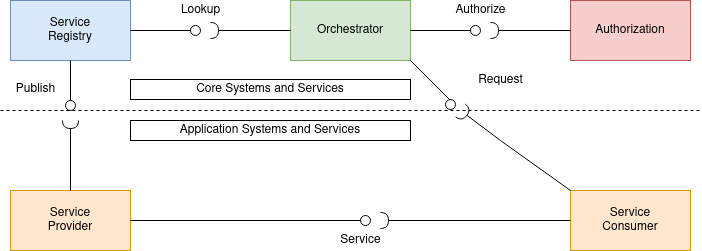
\includegraphics[width=\textwidth]{frames/images/Untitled Diagram.png}
        \end{figure}
\end{frame}

\subsection{Meetings}
The group had two weekly meetings covering the previous week and the status of the project. This structure gave the students a great deal of responsibility to do work for each meeting while still maintaining a good structure of the project and encouraged discussions. 